\section{Shapes}

% \begin{annotate} around an image or table, then \shape lines:
%   \shape<spec>[options]{kind}{x1,y1}{x2,y2}
% Coordinates are fractions of the element (0..1), origin bottom left. The
% grid option (or \showdividers) draws a 0.1 grid to read them off.
% Kinds: rect, ellipse (circle), line, arrow, text ({x,y}{text}).
% Options: color (xcolor: red, green!60!black, ...), width (1pt), fill,
% opacity (0.25), dashed, rounded, label, labelpos (above, below, left,
% right), textsize. Shapes never move anything on the slide.
\begin{frame}{Shapes}{over a figure}
  \begin{columns}[T]
    \begin{column}{0.48\textwidth}
      \begin{figure}
        \begin{annotate}[grid]
          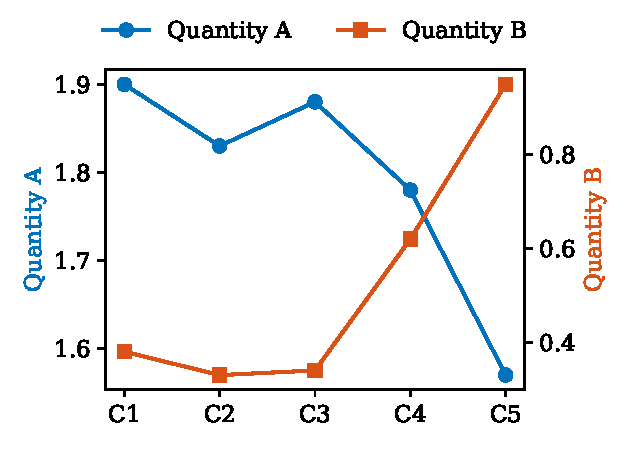
\includegraphics[width=\linewidth]{figures/sample-plot}
        \end{annotate}
        \caption{\texttt{grid}: read off the coordinates.}
      \end{figure}
    \end{column}
    \begin{column}{0.48\textwidth}
      \begin{figure}
        \begin{annotate}
          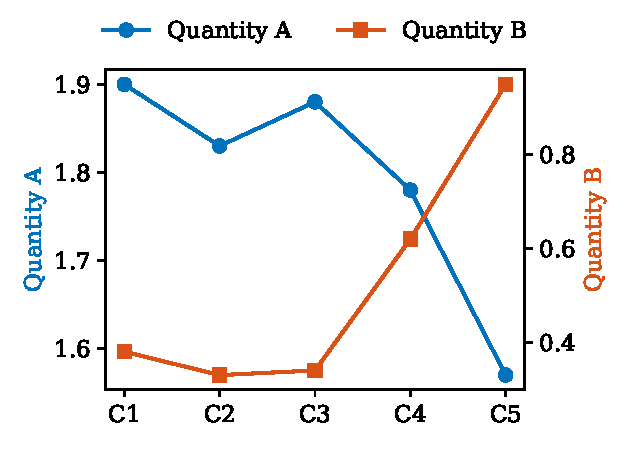
\includegraphics[width=\linewidth]{figures/sample-plot}
          \shape[color=green!60!black]{rect}{0.43,0.12}{0.55,0.84}
          \shape<2->[color=blue, dashed, label=lowest A]{ellipse}{0.75,0.09}{0.86,0.25}
          \shape<3->[color=orange, width=1.5pt]{arrow}{0.25,0.95}{0.42,0.80}
          \shape<3->[color=orange]{text}{0.2,0.97}{selected}
        \end{annotate}
        \caption{\texttt{rect}, then \texttt{ellipse} and \texttt{arrow} on later steps.}
      \end{figure}
    \end{column}
  \end{columns}
\end{frame}

% \slideshape: the same, in fractions of the whole slide (anywhere in a
% frame). \slidegrid shows a grid over the slide while placing them.
\begin{frame}{Shapes}{on the slide}
  \begin{itemize}
    \item \cmd{slideshape} places a shape on the whole slide
    \item \cmd{slidegrid} shows the slide grid while you place it
    \item Use it for callouts that are not tied to one figure
  \end{itemize}
  \slideshape[color=bannerblue, fill=bannerblue, opacity=0.1, rounded,
              label=a slide-level callout, labelpos=below]{rect}{0.55,0.25}{0.92,0.45}
  \slideshape[color=bannerblue, width=1.5pt]{arrow}{0.5,0.62}{0.6,0.47}
  \slidegrid
\end{frame}
